% Options for packages loaded elsewhere
\PassOptionsToPackage{unicode}{hyperref}
\PassOptionsToPackage{hyphens}{url}
\PassOptionsToPackage{dvipsnames,svgnames,x11names}{xcolor}
%
\documentclass[
  letterpaper,
  DIV=11,
  numbers=noendperiod]{scrreprt}

\usepackage{amsmath,amssymb}
\usepackage{iftex}
\ifPDFTeX
  \usepackage[T1]{fontenc}
  \usepackage[utf8]{inputenc}
  \usepackage{textcomp} % provide euro and other symbols
\else % if luatex or xetex
  \usepackage{unicode-math}
  \defaultfontfeatures{Scale=MatchLowercase}
  \defaultfontfeatures[\rmfamily]{Ligatures=TeX,Scale=1}
\fi
\usepackage{lmodern}
\ifPDFTeX\else  
    % xetex/luatex font selection
\fi
% Use upquote if available, for straight quotes in verbatim environments
\IfFileExists{upquote.sty}{\usepackage{upquote}}{}
\IfFileExists{microtype.sty}{% use microtype if available
  \usepackage[]{microtype}
  \UseMicrotypeSet[protrusion]{basicmath} % disable protrusion for tt fonts
}{}
\makeatletter
\@ifundefined{KOMAClassName}{% if non-KOMA class
  \IfFileExists{parskip.sty}{%
    \usepackage{parskip}
  }{% else
    \setlength{\parindent}{0pt}
    \setlength{\parskip}{6pt plus 2pt minus 1pt}}
}{% if KOMA class
  \KOMAoptions{parskip=half}}
\makeatother
\usepackage{xcolor}
\setlength{\emergencystretch}{3em} % prevent overfull lines
\setcounter{secnumdepth}{5}
% Make \paragraph and \subparagraph free-standing
\ifx\paragraph\undefined\else
  \let\oldparagraph\paragraph
  \renewcommand{\paragraph}[1]{\oldparagraph{#1}\mbox{}}
\fi
\ifx\subparagraph\undefined\else
  \let\oldsubparagraph\subparagraph
  \renewcommand{\subparagraph}[1]{\oldsubparagraph{#1}\mbox{}}
\fi


\providecommand{\tightlist}{%
  \setlength{\itemsep}{0pt}\setlength{\parskip}{0pt}}\usepackage{longtable,booktabs,array}
\usepackage{calc} % for calculating minipage widths
% Correct order of tables after \paragraph or \subparagraph
\usepackage{etoolbox}
\makeatletter
\patchcmd\longtable{\par}{\if@noskipsec\mbox{}\fi\par}{}{}
\makeatother
% Allow footnotes in longtable head/foot
\IfFileExists{footnotehyper.sty}{\usepackage{footnotehyper}}{\usepackage{footnote}}
\makesavenoteenv{longtable}
\usepackage{graphicx}
\makeatletter
\def\maxwidth{\ifdim\Gin@nat@width>\linewidth\linewidth\else\Gin@nat@width\fi}
\def\maxheight{\ifdim\Gin@nat@height>\textheight\textheight\else\Gin@nat@height\fi}
\makeatother
% Scale images if necessary, so that they will not overflow the page
% margins by default, and it is still possible to overwrite the defaults
% using explicit options in \includegraphics[width, height, ...]{}
\setkeys{Gin}{width=\maxwidth,height=\maxheight,keepaspectratio}
% Set default figure placement to htbp
\makeatletter
\def\fps@figure{htbp}
\makeatother

\KOMAoption{captions}{tableheading}
\makeatletter
\makeatother
\makeatletter
\@ifpackageloaded{bookmark}{}{\usepackage{bookmark}}
\makeatother
\makeatletter
\@ifpackageloaded{caption}{}{\usepackage{caption}}
\AtBeginDocument{%
\ifdefined\contentsname
  \renewcommand*\contentsname{Table of contents}
\else
  \newcommand\contentsname{Table of contents}
\fi
\ifdefined\listfigurename
  \renewcommand*\listfigurename{List of Figures}
\else
  \newcommand\listfigurename{List of Figures}
\fi
\ifdefined\listtablename
  \renewcommand*\listtablename{List of Tables}
\else
  \newcommand\listtablename{List of Tables}
\fi
\ifdefined\figurename
  \renewcommand*\figurename{Figure}
\else
  \newcommand\figurename{Figure}
\fi
\ifdefined\tablename
  \renewcommand*\tablename{Table}
\else
  \newcommand\tablename{Table}
\fi
}
\@ifpackageloaded{float}{}{\usepackage{float}}
\floatstyle{ruled}
\@ifundefined{c@chapter}{\newfloat{codelisting}{h}{lop}}{\newfloat{codelisting}{h}{lop}[chapter]}
\floatname{codelisting}{Listing}
\newcommand*\listoflistings{\listof{codelisting}{List of Listings}}
\makeatother
\makeatletter
\@ifpackageloaded{caption}{}{\usepackage{caption}}
\@ifpackageloaded{subcaption}{}{\usepackage{subcaption}}
\makeatother
\makeatletter
\@ifpackageloaded{tcolorbox}{}{\usepackage[skins,breakable]{tcolorbox}}
\makeatother
\makeatletter
\@ifundefined{shadecolor}{\definecolor{shadecolor}{rgb}{.97, .97, .97}}
\makeatother
\makeatletter
\makeatother
\makeatletter
\makeatother
\ifLuaTeX
  \usepackage{selnolig}  % disable illegal ligatures
\fi
\IfFileExists{bookmark.sty}{\usepackage{bookmark}}{\usepackage{hyperref}}
\IfFileExists{xurl.sty}{\usepackage{xurl}}{} % add URL line breaks if available
\urlstyle{same} % disable monospaced font for URLs
\hypersetup{
  pdftitle={LANDFIRE-Powered Landscape Assessments},
  pdfauthor={The Nature Conservancy's LANDFIRE team},
  colorlinks=true,
  linkcolor={blue},
  filecolor={Maroon},
  citecolor={Blue},
  urlcolor={Blue},
  pdfcreator={LaTeX via pandoc}}

\title{LANDFIRE-Powered Landscape Assessments}
\author{The Nature Conservancy's LANDFIRE team}
\date{2024-01-09}

\begin{document}
\maketitle
\ifdefined\Shaded\renewenvironment{Shaded}{\begin{tcolorbox}[sharp corners, boxrule=0pt, enhanced, interior hidden, borderline west={3pt}{0pt}{shadecolor}, breakable, frame hidden]}{\end{tcolorbox}}\fi

\renewcommand*\contentsname{Table of contents}
{
\hypersetup{linkcolor=}
\setcounter{tocdepth}{2}
\tableofcontents
}
\bookmarksetup{startatroot}

\hypertarget{background}{%
\chapter*{Background}\label{background}}
\addcontentsline{toc}{chapter}{Background}

\markboth{Background}{Background}

\href{https://landfire.gov/index.php}{LANDFIRE} products are extremely
useful for natural resource managers, allowing users to complete many
tasks, including these that are featured in this website:

\begin{figure}

{\centering 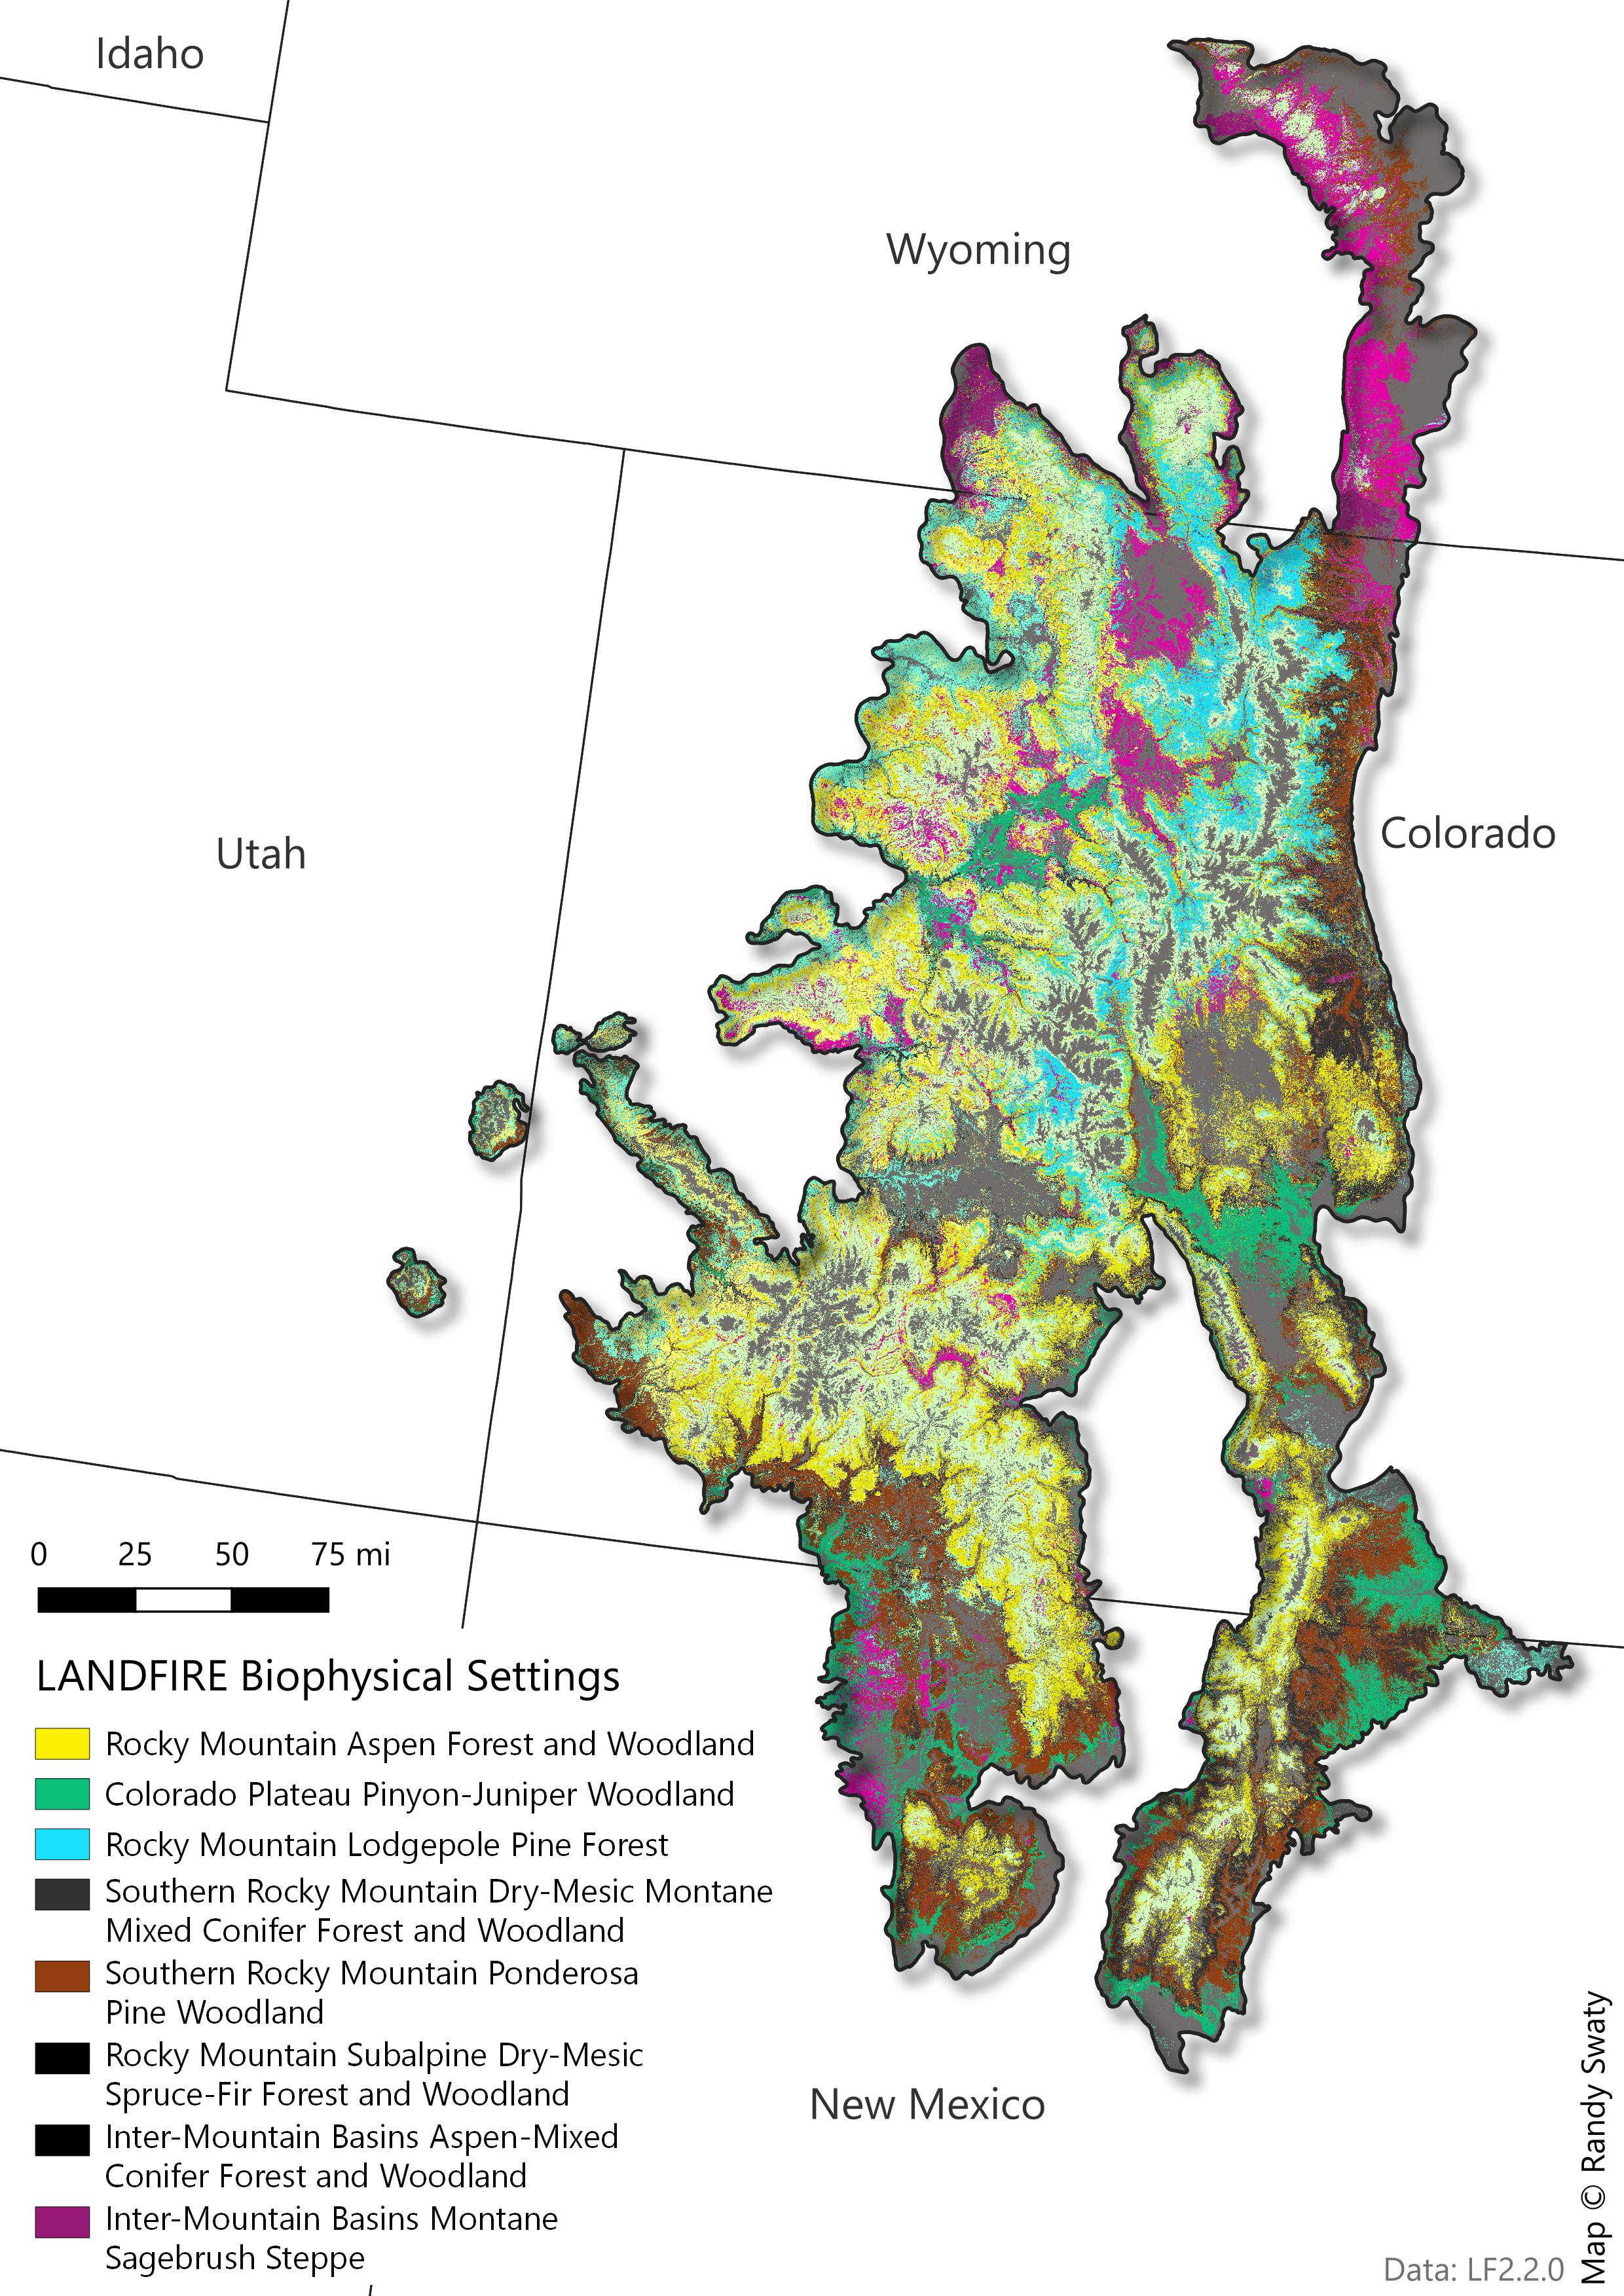
\includegraphics{images/bps.jpg}

}

\caption{Historical ecosystems map.}

\end{figure}

\begin{itemize}
\tightlist
\item
  Mapping and quantifying historical ecosystems (see map below made with
  \href{https://landfire.gov/bps.php}{LANDFIRE's Biophysical Settings
  data})
\item
  Mapping and quantifying existing vegetation type, height and cover
\item
  Comparing reference and current amounts of ecosystem succession
  classes
\end{itemize}

While useful, effectively working with LANDFIRE products can be
intimidating due to terminology, GIS processing and data wrangling often
required.

Additionally, the ``fire-hose'' of information can pose a problem. Where
is a user to start?

\hypertarget{goals}{%
\section*{Goals}\label{goals}}
\addcontentsline{toc}{section}{Goals}

\markright{Goals}

Often a good way to start learning something is to jump in and take on a
meaningful project. Here we show you how to take a shapefile of your
area of interest, then:

\begin{itemize}
\tightlist
\item
  Download and process multiple LANDFIRE datasets
\item
  Bring LANDFIRE data into ArcGIS pro, explore ways to make maps that
  follow Universal Design principles (i.e., easier for everyone to read)
\item
  Quantify and make charts of attributes of interest
\item
  Understand the basics of Biophysical Settings and Models
\end{itemize}

\hypertarget{prerequsites}{%
\section*{Prerequsites}\label{prerequsites}}
\addcontentsline{toc}{section}{Prerequsites}

\markright{Prerequsites}

\hypertarget{the-following-software}{%
\subsection*{The following software}\label{the-following-software}}
\addcontentsline{toc}{subsection}{The following software}

\begin{itemize}
\tightlist
\item
  ArcGIS pro, and basic abilities (e.g., starting a project, bringing in
  data)
\item
  Microsoft Excel (or similar) and/or
  \href{https://cran.rstudio.com/}{R} and
  \href{https://posit.co/download/rstudio-desktop/}{R-Studio}
\item
  SyncroSim
\item
  Microsoft word (or similar)
\end{itemize}

\hypertarget{other}{%
\subsection*{Other}\label{other}}
\addcontentsline{toc}{subsection}{Other}

\begin{itemize}
\tightlist
\item
  A shapefile of your area of interest
\item
  Internet access
\item
  Space to store data
\item
  X\# hours
\end{itemize}

\bookmarksetup{startatroot}

\hypertarget{bps-descriptions}{%
\chapter{BpS Descriptions}\label{bps-descriptions}}

\hypertarget{what-you-will-learn-here}{%
\section{What you will learn here}\label{what-you-will-learn-here}}

A foundational LANDFIRE product are the Biophysical Settings (BpS)
Descriptions and Models. They set the stage for development of many
LANDFIRE products such as the Biophysical Settings and Succession Class
spatial datasets. On this page we will:

\begin{enumerate}
\def\labelenumi{\arabic{enumi}.}
\tightlist
\item
  Learn how to download all of the BpS Descriptions
\item
  Learn how to download one or a set of BpS Descriptions
\item
  Become familiar with:

  \begin{itemize}
  \tightlist
  \item
    The concept of BpS and succession class
  \item
    How LANDFIRE documented `reference conditions' (i.e., how our BpSs
    looked and functioned prior to European colonization)
  \item
    What is contained in the BpS descriptions
  \end{itemize}
\item
  Share links for further learning about BpSs and related topics
\end{enumerate}

\hypertarget{downloading-all-of-the-bps-descriptions}{%
\section{Downloading all of the BpS
descriptions}\label{downloading-all-of-the-bps-descriptions}}

While we typically work with one or a small set of BpSs, there are times
when downloading the entire set developed for the lower 48 states plus
Hawaii and Alaska is most efficient.

\textbf{To download all BpS descriptions:}

\begin{enumerate}
\def\labelenumi{\arabic{enumi}.}
\tightlist
\item
  Navigate to \href{shttps://landfire.gov/bps-models.php}{LANDFIRE's BpS
  Description and Quantitative Models Webpage}
\item
  Scroll down to Download BpS Models and Descriptions Section (see
  below).
\item
  Click on the ``BpS Descriptions'' which will trigger downloading of a
  .zip file named ``LANDFIRE\_CONUS-HI\_BpS\_Descriptions\_Jan2023.zip''
  that has 819 Word Documents. This file will most likely land in your
  ``Downloads'' directory.
\item
  Use your extraction tool of choice to unzip and explore. One possible
  way if you are using Windows is to:

  \begin{itemize}
  \tightlist
  \item
    right click the file
  \item
    select `Extract all' to access the Windows extraction tool (see
    below).
  \end{itemize}
\end{enumerate}

\emph{Where to click to download all BpS descriptions.}

\begin{center}\rule{0.5\linewidth}{0.5pt}\end{center}

\begin{figure}

{\centering 

\href{https://landfire.gov/bps-models.php}{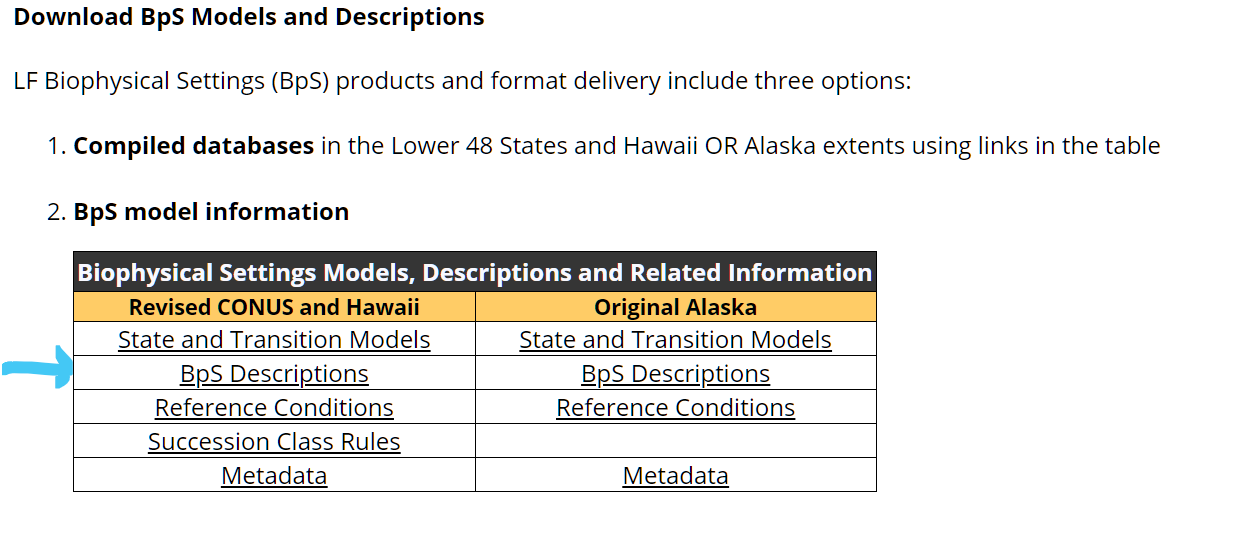
\includegraphics{images/bps_descriptions/download_descriptions_all.png}}

}

\end{figure}

\begin{center}\rule{0.5\linewidth}{0.5pt}\end{center}

\emph{Windows extraction tool being used to unzip all BpS descriptions
file.}

\begin{center}\rule{0.5\linewidth}{0.5pt}\end{center}

\begin{figure}

{\centering 

\href{https://landfire.gov/bps-models.php}{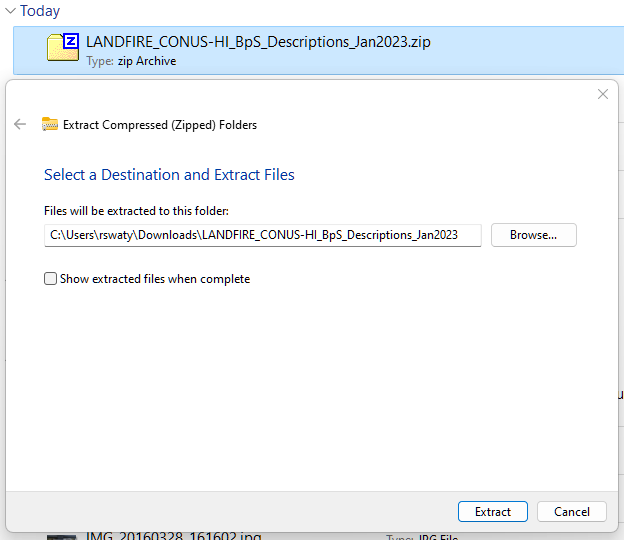
\includegraphics{images/bps_descriptions/zip_click.png}}

}

\end{figure}

\begin{center}\rule{0.5\linewidth}{0.5pt}\end{center}

\hypertarget{downloading-one-or-a-set-of-bps-documents}{%
\section{Downloading one or a set of BpS
documents}\label{downloading-one-or-a-set-of-bps-documents}}

In support of a BpS review process we completed recently, we created a
\href{https://landfirereview.org/}{BpS Models and Descriptions Support}
website, which has a page that allows for searching for, and downloading
a single or a set of BpS Descriptions.

\textbf{To download one or a set of BpS documents}

\begin{enumerate}
\def\labelenumi{\arabic{enumi}.}
\tightlist
\item
  Go to \href{https://landfirereview.org/search.php}{this page} of our
  website.
\item
  There are multiple ways to get BpS documents from here, including:

  \begin{itemize}
  \tightlist
  \item
    Get all BpS documents by one or more broad Vegetation Types (\#1 on
    screenshot below)
  \item
  \end{itemize}
\end{enumerate}

\textbf{Randy's thoughts}

\begin{itemize}
\tightlist
\item
  going over a BpS document is a great way to not only help people
  understand BpS, but also to introduce spatial datasets:

  \begin{itemize}
  \tightlist
  \item
    BpS
  \item
    EVT though s-class rule table (where we get lifeform)
  \item
    EVC and EVH-rule table
  \item
    S-class--look at succession class descriptions to understand what
    ``A'' means in an additional way (in addition to s-class table)
  \end{itemize}
\item
  demo downloading BpS descriptions
\item
  describe key features/sections of document
\item
  link to Blankenship et al 2021
\end{itemize}

\bookmarksetup{startatroot}

\hypertarget{bps-models}{%
\chapter{BpS Models}\label{bps-models}}

\bookmarksetup{startatroot}

\hypertarget{biophysical-settings-models}{%
\chapter{Biophysical Settings
Models}\label{biophysical-settings-models}}

\textbf{Randy's thoughts}

Set people up to use SyncroSim:

\begin{itemize}
\tightlist
\item
  link to veg modeling site
\item
  show how to use LF package
\item
  quick tour of how model connects to description
\end{itemize}

\bookmarksetup{startatroot}

\hypertarget{get-landfire-data}{%
\chapter{Get LANDFIRE data}\label{get-landfire-data}}

\hypertarget{getting-landfire-data-from-the-landfire-map-viewer-lfmv}{%
\section{Getting LANDFIRE Data from the LANDFIRE Map Viewer
(LFMV)}\label{getting-landfire-data-from-the-landfire-map-viewer-lfmv}}

MEGAN does this page.

\hypertarget{randys-ideas}{%
\section{Randy's ideas}\label{randys-ideas}}

\begin{itemize}
\tightlist
\item
  Outline that there are multiple ways (LFMV, streaming, CONUS tifs,
  rlandfire package), and that this page will focus on the LFMV
\item
  Share Jim's videos, noting that things are changing and may look a bit
  different than in the video
\item
  Have directions and screenshots

  \begin{itemize}
  \tightlist
  \item
    turning off the EVT data on the initial opening page so it's easier
    to navigate
  \item
    drawing a rectangle
  \item
    how to select multiple datasets (with links to version description
    page)
  \item
    reminding users to type in email, then to wait (I sometimes forget
    this)
  \item
    etc.
  \end{itemize}
\end{itemize}

\bookmarksetup{startatroot}

\hypertarget{explore-the-spatial-data}{%
\chapter{Explore the spatial data}\label{explore-the-spatial-data}}

\bookmarksetup{startatroot}

\hypertarget{explore-lf-spatial-data-with-arcgis-pro}{%
\chapter{Explore LF spatial data with ArcGIS
Pro}\label{explore-lf-spatial-data-with-arcgis-pro}}

\textbf{Randy's thoughts}

\begin{itemize}
\tightlist
\item
  explore attribute tables of each dataset
\item
  discuss different attributes of EVT and BpS
\item
  limitations of sclass data
\end{itemize}

\bookmarksetup{startatroot}

\hypertarget{make-a-map-with-landfire-data}{%
\chapter{Make a map with LANDFIRE
data}\label{make-a-map-with-landfire-data}}

\bookmarksetup{startatroot}

\hypertarget{make-a-map-with-landfire-data-1}{%
\chapter{Make a map with LANDFIRE
data}\label{make-a-map-with-landfire-data-1}}

\hypertarget{accessibility}{%
\section{accessibility}\label{accessibility}}

\begin{itemize}
\tightlist
\item
  link to Sarah's videos
\item
  highlight challenges
\end{itemize}

\hypertarget{different-maps}{%
\section{different maps}\label{different-maps}}

\begin{itemize}
\tightlist
\item
  EVT
\item
  EVC or EVH
\end{itemize}

\bookmarksetup{startatroot}

\hypertarget{make-charts-with-attribute-data}{%
\chapter{Make charts with attribute
data}\label{make-charts-with-attribute-data}}

\hypertarget{need-and-approach}{%
\section{Need and approach}\label{need-and-approach}}

In addition to the beautiful and useful maps we can make with spatial
data such as delivered by LANDFIRE, it is also useful to summarize the
data. One way to do that is with charts.

Below we will take two approaches: 1) making charts with Datawrapper.de
as it may be new to people, is free and makes nice charts and 2) with R
as it too is free, is easy to replicate and can make nice charts.

\hypertarget{using-datawrapper.de}{%
\section{Using Datawrapper.de}\label{using-datawrapper.de}}

\hypertarget{in-r}{%
\section{In R}\label{in-r}}

\hypertarget{simple-bar-chart-of-bpsevt}{%
\subsection{simple bar chart of
BpS/EVT}\label{simple-bar-chart-of-bpsevt}}

\hypertarget{bar-chart-of-evc-with-custom-colors-though-may-not-match-with-sarahs}{%
\subsection{bar chart of EVC with custom colors (though may not match
with
Sarah's)}\label{bar-chart-of-evc-with-custom-colors-though-may-not-match-with-sarahs}}

\hypertarget{grouped-bar-of-succession-classes}{%
\subsection{Grouped bar of succession
classes}\label{grouped-bar-of-succession-classes}}

\hypertarget{late-succession}{%
\subsection{Late Succession}\label{late-succession}}



\end{document}
